% ALGUNOS PAQUETES REQUERIDOS (EN UBUNTU): %
% ========================================
% %
% texlive-latex-base %
% texlive-latex-recommended %
% texlive-fonts-recommended %
% texlive-latex-extra %
% texlive-lang-spanish (en ubuntu 13.10) %
% ******************************************************** %

\documentclass[a4paper]{article}
\usepackage[spanish]{babel}
\usepackage[utf8]{inputenc}
\usepackage{fancyhdr}
\usepackage[pdftex]{graphicx}
\usepackage{sidecap}
\usepackage{caption}
\usepackage{subcaption}
\usepackage{booktabs}
\usepackage{makeidx}
\usepackage{float}
\usepackage{amsmath, amsthm, amssymb}
\usepackage{amsfonts}
\usepackage{sectsty}
\usepackage{wrapfig}
\usepackage{listings}
\usepackage{enumitem}
\usepackage{hyperref}
\usepackage{listings}
\usepackage{listingsutf8}
\usepackage{enumitem}

% Para ver los marcos
% \usepackage{showframe}

\newcommand{\ord}{\ensuremath{\operatorname{O}}}
\newcommand{\nat}{\ensuremath{\mathbb{N}}}
\renewcommand{\thesubsubsection}{\thesubsection.\alph{subsubsection}}

% Lemas, definiciones, etc.
\theoremstyle{remark}
\newtheorem*{obs}{Observación}
\newtheorem*{nota}{Notación}
\newtheorem*{cor}{Corolario}
\theoremstyle{definition}
\newtheorem*{defi}{Definición}
\theoremstyle{plain}
\newtheorem{teo}{Teorema}
\newtheorem{lema}{Lema}
\newtheorem{prop}{Propiedad}
\usepackage{color} % para snipets de codigo coloreados
\usepackage{fancybox}  % para el sbox de los snipets de codigo

\definecolor{litegrey}{gray}{0.94}

% \newenvironment{sidebar}{%
% 	\begin{Sbox}\begin{minipage}{.85\textwidth}}%
% 	{\end{minipage}\end{Sbox}%
% 		\begin{center}\setlength{\fboxsep}{6pt}%
% 		\shadowbox{\TheSbox}\end{center}}
% \newenvironment{warning}{%
% 	\begin{Sbox}\begin{minipage}{.85\textwidth}\sffamily\lite\small\RaggedRight}%
% 	{\end{minipage}\end{Sbox}%
% 		\begin{center}\setlength{\fboxsep}{6pt}%
% 		\colorbox{litegrey}{\TheSbox}\end{center}}

\newenvironment{codesnippet}{%
	\begin{Sbox}\begin{minipage}{\textwidth}\sffamily\small}%
	{\end{minipage}\end{Sbox}%
		\begin{center}%
		\vspace{-0.4cm}\colorbox{litegrey}{\TheSbox}\end{center}\vspace{0.3cm}}



\usepackage{fancyhdr}
% \pagestyle{fancy}
%\renewcommand{\chaptermark}[1]{\markboth{#1}{}}
\renewcommand{\sectionmark}[1]{\markright{\thesection\ - #1}}
\fancyhf{}
% \fancyhead[LO]{Sección \rightmark} % \thesection\

% \fancyfoot[RO]{\thepage}
\renewcommand{\headrulewidth}{0.5pt}
\renewcommand{\footrulewidth}{0.5pt}
%\setlength{\hoffset}{-0.8in}
\setlength{\textwidth}{16cm}
\setlength{\hoffset}{-1.1cm}
\setlength{\headsep}{0.5cm}
\setlength{\textheight}{25cm}
\setlength{\voffset}{-0.7in}
\setlength{\headwidth}{\textwidth}
\setlength{\headheight}{13.1pt}
\renewcommand{\baselinestretch}{1.1} % line spacing


\begin{document}

\title{Sistemas Operativos}
\author{Manuel Mena}
\maketitle

\tableofcontents

\newpage
\section{Práctica 1}

\subsection{}

Se debe guardar el PCB y los registros del proceso desalojado, y luego cargar
el PCB y los registros del nuevos proceso asignado.

\subsection{}

\begin{codesnippet}
\begin{verbatim}
Ke_context_switch(PCB* pcb_0, PCB* pcb_1) {
    pcb_0->CPU_TIME += ke_current_user_time();
    pcb_0->STAT = KE_READY;
    pcb_0->PC = PC;
    pcb_0->R0 = R0;
    pcb_0->R1 = R1;
    pcb_0->R2 = R2;
    pcb_0->R3 = R3;
    pcb_0->R4 = R4;
    pcb_0->R5 = R5;
    pcb_0->R6 = R6;
    pcb_0->R7 = R7;
    pcb_0->R8 = R8;
    pcb_0->R9 = R9;
    pcb_0->R10 = R10;
    pcb_0->R11 = R011
    pcb_0->R12 = R12;
    pcb_0->R13 = R13;
    pcb_0->R14 = R14;
    pcb_0->R15 = R15;

    PC = pcb_1->PC
    R0 = pcb_1->R0
    R1 = pcb_1->R1
    R2 = pcb_1->R2
    R3 = pcb_1->R3
    R4 = pcb_1->R4
    R5 = pcb_1->R5
    R6 = pcb_1->R6
    R7 = pcb_1->R7
    R8 = pcb_1->R8
    R9 = pcb_1->R9
    R10 = pcb_1->R10
    R11 = pcb_1->R11
    R12 = pcb_1->R12
    R13 = pcb_1->R13
    R14 = pcb_1->R14
    R15 = pcb_1->R15

    pcb_1->STAT = KE_RUNNING;

    ke_reset_current_user_time();
    ret();
}
\end{verbatim}
\end{codesnippet}

\newpage
\section{Práctica 2}

\subsection{}

\subsubsection{}

CPU: [0,2], [11,13], [21,22]
E/S: [3,10], [14,20]

\subsubsection{}

3 y 2 las de CPU, 7 las de E/S

\setcounter{subsection}{3}
\subsection{}

\subsubsection{}

No

\subsubsection{}

Si, que se este ejecutando una tarea de cierta prioridad, llegue una de menor
prioridad que no es atendida, y que a partir de ahí sigan llegando tareas de
mayor prioridad ocasionando que nunca se atienda la tarea de menor prioridad.

\subsubsection{}

Si, que se este ejecutando una tarea de cierta duración, llegue una de mayor
duración que no es atendida, y que a partir de ahí sigan llegando tareas de
menor duración ocasionando que nunca se atienda la tarea de mayor duración.

\subsubsection{}

No

\subsection{}

\subsubsection{}

El efecto es que ese proceso se ejecuta más

\subsubsection{}

Ventaja es que puede discriminarse el quantum de cada proceso, lo cual
permite darle importancia en cierto sentido.

La desventaja es que si se usan múltiples procesadores podría ocurrir que
mientras un procesador este ejecutando una tarea, otro caiga en el PCB
duplicado

\subsubsection{}

Puede utilizarse una lista con los PCB no duplicados y otra con las duraciones
de los quantums de cada proceso.

\setcounter{subsection}{6}
\subsection{}

\subsubsection{}

\begin{tabular}{c c c c c}
Tarea & $T_0$ & $T_1$ & $T_2$ & Promedio \\
Espera & 16 & 21 & 3 & 13.3 \\
Turnaround & 32 & 34 & 24 \\
\end{tabular}

\newpage
\section{Práctica 3}

\subsection{}

\subsubsection{}

No

\subsubsection{}

Puede imprimir 1 en los siguientes casos:

\begin{itemize}
    \item Si se ejecuta primero A y luego B
    \item Si colisionan las ejecuciones de el incremento de X, provocando que
    se ejecuten ambas líneas pero X se incremente sólo una vez
\end{itemize}

Puede imprimir 2 en caso de que se ejecuten B y luego A o que se ejecuten
simultaneamente pero que el printf sea lo último.

\subsection{}

Primero siempre imprime un 0 de la primer X, pero luego como Y ya es 1 puede
imprimir cualquier número de `a's, incluyendo 0, seguido de 1, 2, 3 y 4.

\subsection{}

Primero imprime `b' ya que A se queda haciendo busy waiting sobre X. Luego, es
posible que imprima ``adc'' o ``acd''.

\subsection{}

Si, los procesos acceden y modifican a la variable dentro del mutex, pero lo
liberan y luego toman decisiones respecto a ella, podría producirse una race
condition.

\subsection{}

Podría suceder que se produzca una inanición de los procesos que llaman
primero a wait() ya que quedan en el fondo de la pila hasta que todos los que
llegan después se liberen.

\subsection{}

Supongamos que wait() y signal() no se ejecutaran atómicamente. Supongamos que
tenemos una ejecución de dos procesos y ambos ejecutan wait(). Como wait() no
es atómica una ejecución posible es que ambos procesos lean la capacidad,
salgan del while, y al momento de decrementarla ya están los dos fuera del
ciclo, por lo que ambos ya son capaces de entrar a la zona crítica, violando
el principio de exclusión mutua.

\setcounter{subsection}{7}
\subsection{}

\begin{codesnippet}
\begin{verbatim}
bool TryToLock() {
    return !reg.testAndSet();
}
\end{verbatim}
\end{codesnippet}

\subsection{}

\begin{codesnippet}
\begin{verbatim}
Semaphore semaforos[N] = {0,...,0,1,0,...,0};

for (int j = 0; j < N; j++) {
    int pid = fork();
    if (pid == 0) {
        while (true) {
            semaforos[j].wait();
            P[j];
            semaforos[(j + 1) % N].signal();
        }
    }
}
\end{verbatim}
\end{codesnippet}

\subsection{}

\subsubsection{}

\begin{codesnippet}
\begin{verbatim}
// Semaforos para         A B C
Semaphore semaforos[3] = {1,0,0};

for (int i = 0; i < 3; i++) {
    int pid = fork();
    if (pid == 0) {
        while (true) {
            semaforos[i].wait();
            if(i == 0)
                A();
            else if (i == 1)
                B();
            else if (i == 2)
                C();
            semaforos[(i + 1) % 3].signal();
        }
    }
}
\end{verbatim}
\end{codesnippet}

\subsubsection{}

\begin{codesnippet}
\begin{verbatim}
// Semaforos para         B B C A
Semaphore semaforos[3] = {1,0,0,0};

for (int i = 0; i < 4; i++) {
    int pid = fork();
    if (pid == 0) {
        while (true) {
            semaforos[i].wait();
            if(i == 0 || i == 1)
                B();
            else if (i == 1)
                C();
            else if (i == 3)
                A();
            semaforos[(i + 1) % 4].signal();
        }
    }
}
\end{verbatim}
\end{codesnippet}

\subsubsection{}

\begin{codesnippet}
\begin{verbatim}
// Semaforos para          A  ByC
Semaphore semaforos[2] = { 1 , 0 };

for (int i = 0; i < 3; i++) {
    int pid = fork();
    if (pid == 0) {
        while (true) {
            if(i == 0) {
                semaforos[0].wait(2);
                A();
                semaforo[1].signal(2);
            }
            else if (i == 1) {
                semaforos[1].wait();
                B();
                semaforos[0].signal();
            }
            else if (i == 2) {
                semaforos[1].wait();
                C();
                semaforos[0].signal();
            }
        }
    }
}
\end{verbatim}
\end{codesnippet}

\subsubsection{}

\begin{codesnippet}
\begin{verbatim}
Semaphore sA = Semaphore(1);
Semaphore sB = Semaphore(0);
Semaphore sC = Semaphore(0);

bool sigueB = true;

for (int i = 0; i < 3; i++) {
    int pid = fork();
    if (pid == 0) {
        while (true) {
            if(i == 0) {
                sA.wait(2);
                A();
                if (sigueB) {
                    sigueB = false;
                    sB.signal(2);
                } else {
                    sigueB = true;
                    sc.signal();
                }
            }
            else if (i == 1) {
                sB.wait();
                B();
                sA.signal();
            }
            else if (i == 2) {
                sC.wait();
                C();
                sA.signal(2);
            }
        }
    }
}
\end{verbatim}
\end{codesnippet}

\subsection{}

Se utiliza un contador global. Después de cada $a_i$ se incrementa ese
contador y luego se hace un wait(), pero antes se pregunta si ese proceso es
el último en terminar. Si lo es se hace signal(N) para despertar a todos los
procesos que ya hayan terminado $a_i$. Es necesario utilizar un lock al
incrementar el contador para evitar una race condition. El lock debera abarcar
también la condición para evitar que dos procesos entren con el contador en
el mismo valor.

\begin{codesnippet}
\begin{verbatim}
a();
spin.lock();
cont++;
if (cont == N)
    sem.signal(N);
spin.unlock();
sem.wait();
b();
\end{verbatim}
\end{codesnippet}

\subsection{}

\subsubsection{}

No pueden terminar su ejecución.

\subsubsection{}

No entra en la definición ya que se encuentran esperando a que otros miembros
del grupo liberen el lock.

\subsubsection{}

No puede terminar su ejecución.

\subsubsection{}

Si, entra en la definición ya que se está a la espera de que se libere el
lock.

\subsection{}

\subsubsection{}

No se cumplen las condiciones de Coffman.

\subsection{}

Puede haber deadlock si un recurso toma $R_2$ y los otros dos toman $R_1$, y
todos necesitan ambos recursos para liberar el lock.

Si $R_1$ puede ser compartido por los 3 entonces no puede haber deadlock,
porque el que haya ganado el lock de $R_2$ puede liberarlo al obtener $R_1$, y
así con los 3 procesos.

\subsection{}

No puede haber deadlock ya que como los procesos necesitan a lo sumo dos
recursos, y son todos del mismo tipo, no hay forma de que alguno de los 3
procesos no consigo sus dos recursos, entonces si hay 2 procesos con un
recurso cada uno y el otro con 2, este los libera al terminar y ya los otros
pueden tomar uno cada uno.

\subsection{}

\subsubsection{}

Si, que cada proceso ejecute su primera linea, poniendo ambos semáforos en 0,
para luego atascarse en el wait del semáforo contrario.

\subsection{}

Se puede ver analizándolo proceso a proceso.

\begin{itemize}
\item $P_1$ y $P_3$ ya tienen lo que necesitan por lo que eventualmente
liberarán los recursos asignados: 2$R_2$, 3$R_1$ y 3$R_3$
\item Con eso $P_2$ puede cumplir sus necesidades (2$R_1$ y 2$R_3$) liberando
eventualmente 2$R_1$ y 1$R_4$ además de lo recientemente obtenido
\item Gracias a esto $P_4$ y $P_5$ ya pueden solicitar los recursos que
necesitaban y así terminar su ejecución, habiendo finalizado todos los
procesos
\end{itemize}

\subsubsection{}

Si, hay deadlock. Anteriormente ocurría que $P_1$ y $P_3$ liberarían los
recursos obtenidos ya que ya habían satisfacido sus necesidades, pero en este
caso $P_3$ todavía necesita 2$R_2$. El único que puede liberar recursos es
$P_1$, pero como libera únicamente 1$R_2$, esto no alcanza para satisfacer a
$P_3$ y por lo tanto $P_2$, $P_3$, $P_4$ y $P_5$ quedan a la espera de que se
les asigne sus respectivos recursos, sin liberarlos nunca.

\subsection{}

\subsubsection{}

\begin{codesnippet}
\begin{verbatim}
a();
spin.lock();
cont++;
if (cont == N)
    sem.signal(N);
spin.unlock();
sem.wait();
b();
\end{verbatim}
\end{codesnippet}

\subsubsection{}

\begin{codesnippet}
\begin{verbatim}
a();
atomReg.inc();
while(atomReg.get() != N) {}
b();
\end{verbatim}
\end{codesnippet}

\subsubsection{}

\begin{codesnippet}
\begin{verbatim}
a();
if (atomReg.getAndInc() == N - 1)
    sem.signal(N);
sem.wait();
b();
\end{verbatim}
\end{codesnippet}

\subsubsection{}

La más fácil de entender es en la que se usan sólo el registro atómico debido
a su simpleza.

\subsubsection{}

La más eficiente es la tercera ya que no desperdicia tiempo haciendo busy
waiting como las otras dos.

\subsection{}

\begin{codesnippet}
\begin{verbatim}
// Variables globales:
atomic<int> clientesDentro;

queue<Sempaphore cliente> colaLocal;
queue<Sempaphore cliente, Semaphore barbero> colaSofa;

TasLock lockLocal;
TasLock lockSofa;
TasLock lockPagando;

Semaphore quieroPagar, aceptoPago, pagoAceptado;
int esperandoAPagar;

// Cliente:

Semaphore yo = new Semaphore(0);
Semaphore barbero = new Semaphore(0);

// Si el local está lleno me voy al chori
if (clientesDentro.getAndInc() > 20) {
    clientesDentro.getAndDec();
    exit();
}

lockLocal.lock();
colaLocal.push(yo);
lockLocal.unlock();
entrar();

// Si hay espacio en el sofa voy y me siento
lockSofa.lock();
if (colaSofa.size() < 4) {
    lockLocal.lock();
    colaLocal.pop();
    colaSofa.push(<yo, barbero>);
    sentarseEnSofa();
    lockLocal.unlock();
    lockSofa.unlock();
} else {
    lockSofa.unlock();

    // Espero a que me llamen cuando se desocupe un lugar en el sofa
    yo.wait();

    // Me despertaron, me siento en el sofa
    lockSofa.lock();
    lockLocal.lock();
    colaLocal.pop();
    colaSofa.push(<yo, barbero>);
    sentarseEnSofa();
    lockLocal.unlock();
    lockSofa.unlock();
}

// Espero a que el barbero me llame
yo.wait();

\end{verbatim}
\end{codesnippet}

\begin{codesnippet}
\begin{verbatim}

lockSofa.lock();

// Si el sofa estaba lleno tengo que avisarle al proximo que se siente
if (colaSofa.size() == 3) {
    parado.signal();
}

lockSofa.unlock();

sentarmeEnSilla();
barbero.signal();

// Espero a que el barbero termine de cortarme el pelo
yo.wait();

// Se terminó el corte, voy a pagar
lockPagando.lock();
esperandoAPagar++;
lockPagando.unlock();
quieroPagar.wait();

// Pago
pagar();
aceptoPago.signal();
pagoAceptado.wait();

// Pago aceptado, salgo
clientesDentro.getAndDec();
salir();
exit();

// Barbero:

Semaphore yo, cliente;

while(true) {
    lockSofa.lock();
    if (!colaSofa.empty()) {
        <Semaphore,Sempahore> sentado = colaSofa.top();
        colaSofa.pop();

        cliente = sentado.cliente;
        yo = sentado.barbero;

        // Le aviso al cliente que venga a ser atendido
        cliente.signal();

        // Espero a que el cliente se siente en la silla
        lockSofa.unlock();
        yo.wait();

        // El cliente se sienta
        cortarCabello();

\end{verbatim}
\end{codesnippet}

\begin{codesnippet}
\begin{verbatim}

        //Le aviso que termine de cortar el pelo
        cliente.signal();
    } else
        lockSofa.unlock();

    lockPagando.lock();
    if (esperandoAPagar > 1) {
        esperandoAPagar--;
        lockPagando.unlock();

        // Le aviso a alguno que puede pagar
        quieroPagar.signal();

        // Espero a que me paguen
        aceptoPago.wait();

        // Me pagan
        aceptoPago();
        pagoAceptado.signal();
    } else
        lockPagando.unlock();
}
\end{verbatim}
\end{codesnippet}

\subsection{}

\begin{codesnippet}
\begin{verbatim}
Semaphore semMacho[N] = {0,...,0}
Sempahore semHembra[N] = {0,...,0};

void P(i, sexo) {
    if (sexo == macho) {
        semMacho[i].signal();
        semHembra[i].wait();
    } else {
        semHembra[i].signal();
        semMacho[i].wait();
    }
    entrar(i);
}
\end{verbatim}
\end{codesnippet}

\newpage
\section{Práctica 4}

\subsection{}

Una dirección de memoria lógica es traducida a una de memoria lineal a
través de la segmentación, y ésta es traducida a una dirección de memoria
física mediante la paginación.

\subsection{}

Fragmentación interna es cuando los bloques son muy grandes para los datos
almacenados dentro de ellos, lo que provoca que se desperdicie espacio.
Fragmentación externa es cuando no hay suficiente memoria contigua para ser
asignada, por lo que queda inutilizable.

\subsection{}

Bloques
\begin{enumerate}
	\item 8MB 2MB
	\item 1MB
	\item 4MB 1MB
	\item 512KB 12KB
	\item 512KB
	\item 2MB
\end{enumerate}

Programas
\begin{enumerate}
	\item 500KB
	\item 6MB
	\item 3MB
	\item 20KB
	\item 4MB
\end{enumerate}

\subsubsection{}

\begin{itemize}
	\item Programa 1 en bloque 4
	\item Programa 2 en bloque 1
	\item Programa 3 en bloque 3
	\item Programa 4 en bloque 2
	\item Programa 5 en bloque 1
\end{itemize}

\subsection{}

Porque con una dirección lineal de $n$ cantidad de bits pueden direccionarse
$2^n$ páginas, por lo que una la tabla tiene $2^n$ entradas.

\setcounter{subsection}{6}
\subsection{}

65536 bytes divididos en páginas de 4096 bytes hacen 16 páginas en total. Se
necesitan 8 páginas para el texto, 5 para los datos y 4 para la pila, por lo
que no es posible ejecutarlo.

Si el tamaño de página fuera de 512 bytes, se tendrían direccionadas 128
páginas. El texto del programa requeriría 64, los datos 33 y la pila 31. De
esta forma sí podria ejecutarse.

\subsection{}

\subsubsection{}

400, porque se debe acceder primero a la entrada correspondiente de la tabla y
una segunda vez para la página.

\subsection{}

Ocurre cuando se intenta acceder a una página que ya no está en memoria. Lo
que el sistema hace en ese caso es guardar en disco una de las páginas ya
cargadas en memoria para hacer espacio a la página que se está intentando
acceder. Una vez hecho esto se lee la página de disco y se la carga en
memoria.

\setcounter{subsection}{10}
\subsection{}

\subsubsection{}

Cada pagina contiene 200 posiciones por lo que habrá 50 fallos de página

\subsubsection{}

Como la matriz está almacenada contiguamente por por fila, este tipo de
recorrido salta a través de las columnas, por lo que cada pagina solo
albergará 2 posiciones, por lo que habran 5000 fallos de página

\setcounter{subsection}{12}
\subsection{}

\subsubsection{}

Tiene sentido si lo que se hace es dejar un segmento especialmente para
atender las llamadas. Si fuese parte de la paginación, sería posible que la
página en donde está almacenado el código para la atención de llamadas se
encuentre fuera de memoria, por lo que se perdería tiempo en traerla de disco.

\subsubsection{}

Si, justamente para ahorrarse el tiempo de ir a buscarlas a memoria.

\newpage
\section{Práctica 5}

\subsection{}
Son necesarios $N$ accesos a memoria.

\subsection{}

\subsubsection{}
Es necesario leer los primeros 10 bloques directos.

\subsubsection{}
Es necesario leer los 12 bloques directos, el bloque de indirección simple y
los primeros 8 bloques del bloque de indirección. 21 en total.

\subsection{}

\subsubsection{}

\subsubsection{}
Conviene usar inodos ya que FAT no está acotado.

\subsubsection{}
Conviene usar FAT ya que mediante inodos esta acotado por la cantidad de
bloques del inodo.

\subsubsection{}
Conviene usar inodos porque se carga un inodo y los bloques del archivo a
medida que se van leyendo, en FAT se debe cargar la tabla entera a memoria.

\subsection{}

\subsubsection{}
Los identificadores de bloque son de 24 bits, por lo que es posible
direccionar hasta $2^{24}$ bloques. El del hash es de 16 bits por lo que el
tamaño de la tabla es de $2^{16}$ entradas.

La FAT contiene solo identificadores de bloque de 24 bits, por lo que su
tamaño es de $2^{24} \times 24$ bits. Lo que es lo mismo que
$2^{24} \times 3$ bytes $= 48MiB$.

En cuanto a la tabla de hash, cada entrada contiene el identificador de bloque
(24 bits) y el tamaño del archivo. El tamaño de un archivo no está actotado,
por lo que en principio podría llegar a ser de 16GiB, que es el tamaño del
disco. Por lo que para almacenar el tamaño del archivo se necesitan 34 bits,
siendo un total de 58 bits por entrada. El tamaño de la tabla de hash es de
$2^{16} \times 58$ bits $= 3801088$ bits $=14848$ bytes, poco más de 14KiB.

Como el tamaño de bloque es de dos sectores, y cada sector de 1KiB, la unidad
mínima es de 2KiB. La FAT queda almacenada a la perfección en 24Ki sectores,
pero el hash no, por lo que sufre de un poco de fragmentación interna; se
necesitan 7 bloques para cubrir 14KiB y un bloque extra para el resto.

Ambas estructuras ocupan entonces 24Ki + 8 bloques, lo que equivale a 50348032
bytes. Quedando mas de 15,95 Gib para los archivos.

\subsubsection{}
El tamaño del bloque debería ser de 2 sectores, ya que es lo que mejor se
ajusta al tamaño de los archivos, por mas que se desperdicie la mitad de la
memoria. Esto hace que la cantidad de bloques posibles a ser direccionados sea
de $\frac{16GiB}{2KiB} = 8Mi$ bloques $= 2^23$ bloques. Por lo que se
necesitan 23 bits para direccionarlos, lo cual genera la necesidad de que el
tamaño de los identificadores de bloque sea de 24 bits. Por último, como cada
archivo requerirá en promedio 1 bloque, puede decirse que se tiene la misma
cantidad de archivos que de bloques, entonces el tamaño del hash también es de
24 bits.

\subsubsection{}
En caso en que los archivos tuviesen un tamaño promedio de 16MiB, uno
intentaría usar el tamaño máximo de bloque que es de 8 sectores (8 KiB). Pero
la cantidad de bits a utilizar para los identificadores de bloque diferiría
en 2 (o en 1 si se usasen bloques de 4 sectores), lo cual lleva a utilizar la
configuración de 24 bits de todos modos, y lo mismo para el hash.

\subsection{}
Si, en caso en que varios procesos intenten leer el mismo bloque, con raid 0
deberán turnarse para leerlo, mientras que con raid 1 cada proceso puede leer
una copia distinta.

\subsection{}

\subsubsection{}
2 accesos: el bloque a escribir y el de paridad.

\subsubsection{}
9 accesos: 7 para los bloques, 1 para la paridad de los primeros 4 y otro para
la de los últimos 3.

\setcounter{subsection}{7}
\subsection{}

\subsubsection{}
Falso, siempre puede incrementarse el nivel de protección agregando una copia
más, en caso de que el resto de las copias fallen.

\subsubsection{}
La aumenta en el sentido de que esa cinta puede ser robada, pero también puede
ser robado el disco en donde está almacenada la información, y de hecho es más
vulnerable dentro del disco ya que es posible que sea accedido de manera
remota, lo cual no ocurre con la cinta.

\subsection{}
Un snapshot es una imágen del estado del sistema, una forma de recuperar

\newpage
\section{Práctica 6}

\subsection{}
Polling sería más conveniente en caso de que se realice una comunicación
constante, para cualquier caso en que se envíe una ráfaga de datos es mucho
más costoso el tiempo perdido en cambios de contexto si se implementara el
uso de interrupciones que el tiempo de espera activa del polling.

Si la comunicación tuviese intervalos largos o no determinados, conviene la
estrategia de interrupciones, como en un teclado.

El caso híbrido es el que se envían ráfagas de datos separadas por intervalos
largos. Se utilizan las interrupciones para establecer la comunicación, se
envía la ráfaga de datos atendida mediante polling, y una vez finalizada se
espera a la próxima interrupción.

\subsection{}
El uso de E/S de un procesos en promedio es de 0.77, entonces el uso de la CPU
para 6 procesos es

\begin{center}
$U_{CPU}(6) = 1 - U_{E/S}(1)^6 = 1 - 0.2084 = 0.7916$
\end{center}

En cuanto al DMA,

\begin{center}
$U_{DMA}(6) = 1 - U_{CPU}(1)^6 = 1 - 0.23^6 = 0,9998$
\end{center}

\subsection{}

\subsubsection{}
La velocidad de los dispositivos virtuales va a ser la misma que la de los
procesos, no?

\subsubsection{}
La latencia mejora ya que los procesos no necesitan quedarse esperando a que
el dispositivo esté listo.

La liberación de recursos es mayor ya que no se hace espera activa.

El throughput mejora porque es posible usar los recursos liberados para otras
tareas.

\subsection{}

\subsubsection{}
Debe estar al tanto de que haya spooling.

\subsubsection{}
El driver no sabe que hay o no spooling, solo el usuario.

\subsection{}

\subsubsection{}
Si, el driver es código.

\subsubsection{}
No, el driver es solamente software.

\subsubsection{}
No. Es una porción de software hecha por el fabricante del dispositivo a
controlar.

\subsubsection{}
No, se ejecuta en espacio de kernel.

\subsubsection{}
Falso. Además de interrupciones, puede trabajar mediante polling o DMA.

\subsubsection{}
Verdadero?

\subsection{}
\begin{codesnippet}
\begin{verbatim}
int driver_init() {}
int driver_remove() {}
int driver_open() {}
int driver_close() {}

int driver_read(int *data) {
    *data = IN(CHRONO_CURRENT_TIME);
    return IO_OK;
}

int driver_write(int *data) {
    OUT(CHRONO_CTRL, CHRONO_RESET);
    return IO_OK;
}
\end{verbatim}
\end{codesnippet}

\subsection{}

\setcounter{subsection}{10}
\subsection{}

\subsubsection{}
\begin{codesnippet}
\begin{verbatim}
int write(int sector, void *data) {
    if (DOR_STATUS)
        OUT(DOR_IO, 1);
    sleep(50);

    OUT(ARM, sector / cantidad_sectores_por_pista());
    while(ARM_STATUS) {}

    OUT(SEEK_SECTOR, sector % cantidad_sectores_por_pista());

    escribir_datos(data);
    while(DATA_READY) {}
}
\end{verbatim}
\end{codesnippet}

\subsubsection{}
\begin{codesnippet}
\begin{verbatim}
Semaphore ready;
Semaphore timer;

void arm_or_data_ready() {
    ready.signal();
}

void timer_ready() {
    timer.signal();
}

int driver_init() {
    ready = new Sempaphore(0);
    timer = new Sempaphore(0);
    request_irq(6, arm_or_data_ready);
    request_irq(7, timer_ready);
}

int write(int sector, void *data) {
    if (DOR_STATUS)
        OUT(DOR_IO, 1);
    timer.wait();

    OUT(ARM, sector / cantidad_sectores_por_pista());
    ready.wait();

    OUT(SEEK_SECTOR, sector % cantidad_sectores_por_pista());

    escribir_datos(data);
    ready.wait();

    return(IO_OK);
}
\end{verbatim}
\end{codesnippet}

\newpage
\section{Práctica 7}

\subsection{}

\subsubsection{}
Se aplica la función de hash a la contraseña que ingresó el usuario y si el
resultado coincide con el valor almacenado entonces el ingreso es exitoso.

\subsubsection{}
La probabilidad de acertar con una contraseña distinta es de $\frac{1}{2^64}$.

\subsubsection{}
Cantidad de contraseñas a probar: $2^63$.

Cantidad de contraseñas por segundo: $10^9$.

Cantidad de segundo por año: $3.15 \times 10^7$.

Serían necesarios $\frac{2^63}{10^16 \times 3.15} ~= 293$ años.

\subsubsection{}
Cantidad de contraseñas a probar: $36^6$.

Cantidad de contraseñas por segundo: $10^9$.

Serían necesarios $\frac{36^6}{10^9} = 2.18$ segundos.

\subsection{}

\subsubsection{}
No es seguro ya que es vulnerable a un replay-attack. Consiste en interceptar
la información y retransmitirla, haciéndose pasar por otra persona.

\subsubsection{}
El atacante tendría el seed y el hash, lo que podría hacer es hashear todas
las contraseñas posibles con ese seed hasta que coincida con el hash robado.
Pero para eso necesitaría tener la función de hash.

\subsection{}

\subsubsection{}
El problema se introduce en la funcion \textit{gets}, puesto que esta no se
fija que la entrada tenga menor tamaño que la variable a donde se almacenará,
y como consecuencia el contenido pisa el resto de la pila de la función
pudiendo pisarse la dirección de retorno, desencadenando la ejecución de otro
programa almacenado en otra posición de memoria.

\subsubsection{}
Únicamente la variable nombre.

\subsubsection{}
La dirección de retorno de \textit{gets} si.

\subsubsection{}
No. Una vez que se llama a \textit{gets} el usuario ya tomó el control.

\subsection{}
Primero se apilan los parámetros de \textit{login}, luego la dirección de
retorno y finalmente las variables locales, que en este caso son un arreglo de
char de 32 posiciones y un credential que contiene otros 2 arreglos de char de
32 posiciones cada uno.

Las variables se apilan de manera tal que al leerlas o escribirlas se hace
descendiendo por la pila. El problema es que \textit{fgets} puede escribir
hasta la cantidad de caracteres que se pasa por parámetro, y en este caso es
errónea ya que debería ser \textit{sizeof(user.pass)} en lugar de
\textit{sizeof(user)}. Esto permite que puedan escribirse los siguientes 32
bytes de la pila, que en el caso del segundo \textit{fgets}, es el espacio
reservado para la contraseña real. Y asi puede sobreescribirse en la pila la
verdadera contraseña y engañar al programa.

\subsubsection{}
Los valores son \textit{admin} para el usuario, y
\textit{cualquiercontraseñad32caracterescualquiercontraseñad32caracteres} para
la contraseña.

\subsection{}

\subsubsection{}
El mecanismo que hace esto posible es el parámetro setUid a la hora de asignar
los permisos del ejecutable de este código. Se establece que este programa que
puede ser ejecutado por cualquier usuario, tiene permisos para abrir o
ejecutar otros archivos como si fuera root.

\subsubsection{}
El problema está en que \textit{gets} puede sobreescribir la dirección de
retorno si el string que se pasa tiene mas de 128 caracteres. Puede controlar
todo lo que este apilado debajo de la contraseña.

\subsection{}

\subsubsection{}
Si. Si lo que se le pasa a la funcion es un NaN.

\subsubsection{}
Podría devolver 0 en caso en que se le pase un NaN.

\setcounter{subsection}{7}
\subsection{}

\subsubsection{}
. ; cat /etc/passwd

\subsubsection{}
Puede pasarsele: .'' ; cat ''/etc/passwd

\subsubsection{}
Puede pasarsele: .'' \&\& cat ''/etc/passwd

\subsubsection{}
\begin{codesnippet}
\begin{verbatim}
void wrapper_ls(const char * dir) {
    pid_t pid = fork();
    if (pid == 0) {
        execve(``ls'', dir);
    } else {
        int status;
        while (waitpid(pid, &status, 0) == -1) {}
    }
}
\end{verbatim}
\end{codesnippet}

\newpage
\section{Preguntas de finales}

\subsection{Marzo 2020}
\subsubsection{Procesos - Explicar diferencia entre proceso y thread y relación de este último con funciones reentrantes. Explicar qué es un árbol de procesos y cuál es su importancia}


Un proceso es un programa en ejecución. El proceso puede invocar tantos threads como necesite, cada thread corresponde a un único proceso. En algunas implementaciones, los recursos de los threads se distribuyen entre los recursos totales de su proceso padre, lo cual esta descripto por el árbol de procesos, y en otras pueden asignarseles recursos independientemente.

Cada proceso se refleja en un bloque de una tabla llamado Process Control Block (PCB), el cual cuenta con la información necesaria para identificar al proceso univocamente (pid) junto con data del proceso que describe el estado del proceso en el momento en que es pausado (estado, program counter, archivos abiertos, registros, stack), para asi poder reanudarlo cuando se desee y resulte transparente al proceso.

En una implementacion con threads se requiere ampliar esta implementacion de la tabla de PCB adjuntando un identificador del thread (tid), el pid del proceso al que pertenece y tambien data que permita determinar el estado de la ejecución, de la misma manera que con los procesos.

Los threads son una forma de paralelizar la ejecución de un proceso, ya sea para poder tener varias responsabilidades simultaneamente o para dividir un problema en partes y poder atacarlo mas rapidamente.

Una función reentrante es aquella que garantiza que multiples instancias de la misma pueden ejecutarse simultaneamente sin que eso provoque una falla en el sistema. Si una función fuese a ser ejecutada por distintos threads, y no hay garantías de que lo vayan a hacer de manera exclusiva, entonces esta debe ser necesariamente reentrante.

\subsubsection{Sincronización - Explicar deadlock con un dibujo y en pocas palabras}

Las $P$ son procesos y las $R$ recursos

Arcos:
\begin{itemize}
\item De $P$ a $R$, $P$ requiere $R$
\item De $R$ a $P$, $P$ adquirió $R$
\end{itemize}

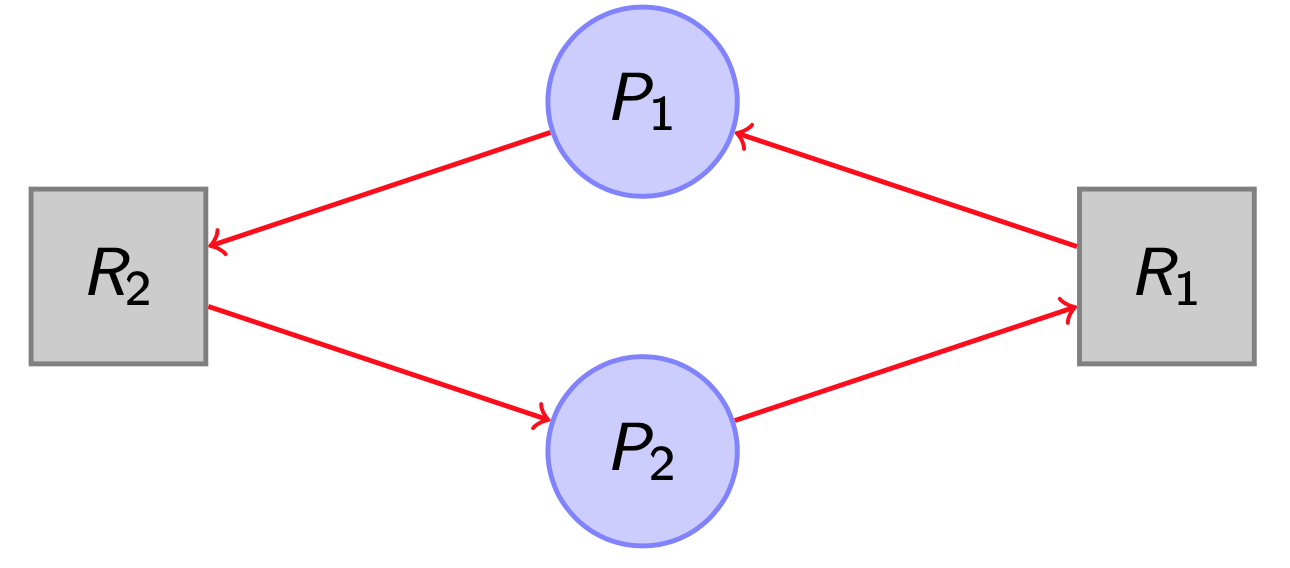
\includegraphics[width=0.6\textwidth]{imagenes/deadlock}

\subsubsection{Administración de E/S - ¿Por qué los algoritmos de scheduling se miden en cilindros? ¿Está bien? ¿Por qué? Explicar SAN}
Se llama \textit{seek time} al tiempo que tarda el brazo de un HDD en transportar los cabezales al cilindro correspondiente. El tiempo de accesso depende mayormente del \textit{seek time} y de la latencia de rotación.

Los algoritmos de scheduling de E/S definen de qué manera se moverá el brazo del disco lo cual determina el orden en que se atenderán los pedidos, en función del número de cilindro de cada uno. Cuanta más distancia recorra el brazo para cumplir los pedidos, mayor será el \textit{seek time} y más tardará en completarlos. Se miden en cilindros porque es la unidad de distancia del movimiento del brazo, cuanto mejor estén ordenados los pedidos, menos cilindros el brazo tendrá que recorrer para servirlos y mejor será el tiempo hasta completarlos.

SAN significa Storage Area Network. Se trata de tener el almacenamiento en la red, pero una red especial, donde los protocolos son específicos para este tipo de datos (son de más bajo nivel). 

El problema de tener Network Attached Storage (NAS) es que las operaciones consumen ancho de banda repercutiendo en la comunicación de la red.

\subsubsection{Seguridad - Explicar qué es una función de hash segura y ejemplificar dos usos en un sistema operativo. - comparar DAC y MAC}

Una función de hash segura es aquella que tiene muy baja probabilidad de generar colisiones y que sea muy difícil de revertir, es decir, sabiendo $y$ encontrar $x$ siendo $f(x) = y$, con $f$ la función de hash.

Discretionary Access Control (DAC): El acceso se controla basandose en las identidades de los usuarios y grupos. Se puede implementar con una matriz donde se almacena para cada sujeto, los distintos permisos sobre cada objeto. Los atributos de seguridad se definen explicitamente (se puede hacer solamente lo que está especificado). Es el usuario dueño del archivo quien determina quiénes tienen acceso al mismo.

Mandatory Access Control (MAC): Cada sujeto tiene un grado (se suele manejar el concepto de label). Los objetos heredan el grado/label del último sujeto que los modificó. Un sujeto sólo puede acceder a objetos de grado igual o menor que el suyo.

\subsubsection{Filesystems - Explicar journaling en ext3. ¿Qué problema resuelve?}

Cuando el sistema quiere realizar una transacción, en lugar de realizarla inmediatamente, se la escribe en el \textit{journal}. A esto se lo llama realizar un \textit{commit}. Un vez hecho el \textit{commit}, se devuelve el control al proceso usuario mientras el filesystem hace el replay de los commits registrados.

Este otro proceso mantiene un puntero que indica la operación dentro del commit que se está llevando a cabo, el cual va moviendo a medida que va satisfaciendo las operaciones y con ellas, los commits. Este algoritmo permite que ante una falla completa del sistema que requiera un reinicio, se pueda consultar el \textit{journal} para asi reestablecer el sistema mediante el puntero, y continuar con la operación que habia quedado pendiente, asi como con el resto de los commits que aún no habían sido ejecutados.
\end{document}
